% CMG-PES residual control architecture, final version (2026-10-01).
% Same visual language as the manuscript's architecture_standalone.pdf (arch_style.tex), with the signal flow checked
% against equations (3)-(28) and the code (run_final_robustness.py, nengo_cmg.py):
%   * the saturation-aware gate (28) is an explicit block; it reads u_0 and passes s~ to the bounded addition (27)
%   * the nominal law is the PD + desired-rate feedforward of (15); the reference supplies q_d and omega_d
%   * PES learns from the pre-gate decoder output s_k (the gate masks the output only, never the update)
%   * every interval limit is written sat, as in the updated manuscript text
%   pdflatex architecture_cmg_pes.tex   ->  architecture_cmg_pes.pdf (use in the paper as figure*, width 0.9\textwidth)
\documentclass[border=4pt,tikz]{standalone}
\usepackage{amsmath,amssymb,bm}
\usetikzlibrary{arrows.meta,positioning,fit,backgrounds,calc}
\newcommand{\T}{^{\mathsf T}}
\newcommand{\sat}{\operatorname{sat}}
\newcommand{\sgnp}{\operatorname{sgn}_{+}}
% Shared TikZ style for all architecture figures. Grayscale-safe.
\tikzset{
  blk/.style   ={draw,rounded corners=2pt,align=center,font=\footnotesize,
                 minimum height=8mm,inner sep=3pt,fill=white},
  clas/.style  ={blk,fill=black!4},
  neuro/.style ={blk,fill=black!12,very thick},
  plant/.style ={blk,fill=black!20},
  meas/.style  ={blk,dashed},
  sum/.style   ={draw,circle,inner sep=0pt,minimum size=4.5mm,font=\scriptsize},
  sig/.style   ={-{Latex[length=2mm]},thick},
  sigd/.style  ={-{Latex[length=2mm]},thick,dashed},
  lbl/.style   ={font=\scriptsize,inner sep=1.5pt,fill=white},
  grp/.style   ={draw,dashed,rounded corners=3pt,inner sep=6pt},
  note/.style   ={font=\scriptsize\itshape,align=left},
}

\tikzset{
  blk/.append style={font=\footnotesize,inner sep=3.5pt},
  gatek/.style={blk,fill=orange!10,draw=orange!60!black,thick},
}
\begin{document}
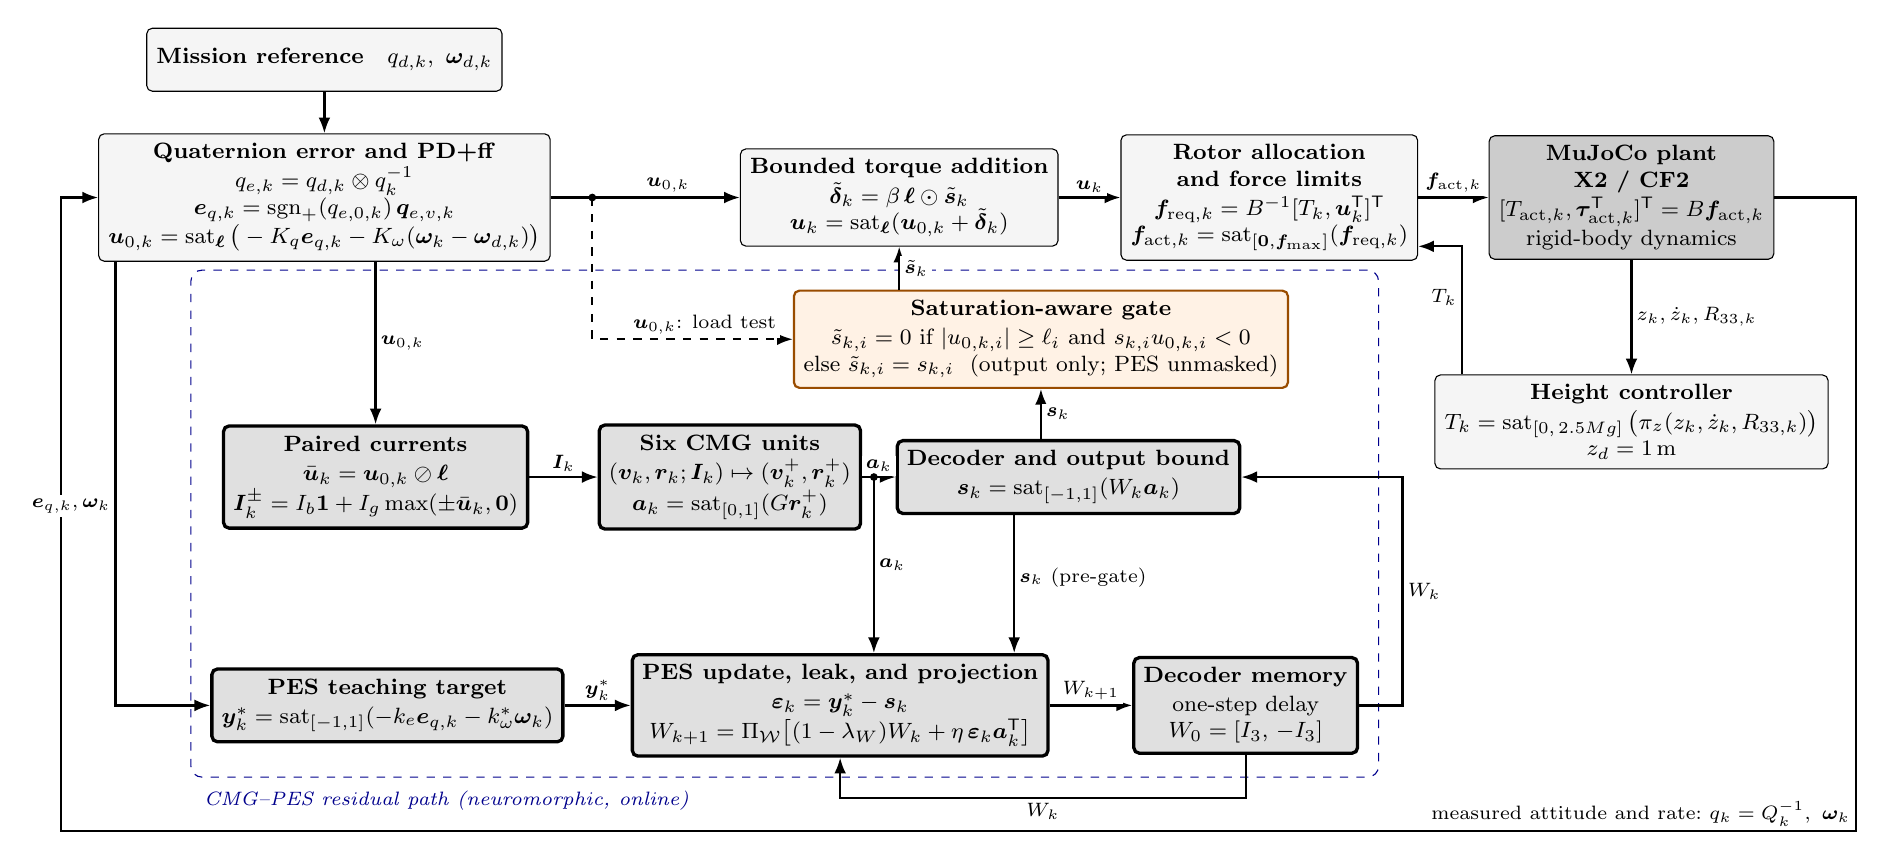
\begin{tikzpicture}[x=1cm,y=1cm]
  % ------------------------------------------------------------------ classical loop (top row)
  \node[clas] (ref) at (2.6,1.75) {\textbf{Mission reference}\quad $q_{d,k},\ \bm\omega_{d,k}$};
  \node[clas] (pd) at (2.6,0) {\textbf{Quaternion error and PD+ff}\\[1pt]
      $q_{e,k}=q_{d,k}\otimes q_k^{-1}$\\
      $\bm e_{q,k}=\sgnp(q_{e,0,k})\,\bm q_{e,v,k}$\\
      $\bm u_{0,k}=\sat_{\bm\ell}\big(-K_q\bm e_{q,k}-K_\omega(\bm\omega_k-\bm\omega_{d,k})\big)$};
  \node[clas] (add) at (9.9,0) {\textbf{Bounded torque addition}\\[1pt]
      $\tilde{\bm\delta}_k=\beta\,\bm\ell\odot\tilde{\bm s}_k$\\
      $\bm u_k=\sat_{\bm\ell}(\bm u_{0,k}+\tilde{\bm\delta}_k)$};
  \node[clas] (alloc) at (14.6,0) {\textbf{Rotor allocation}\\\textbf{and force limits}\\[1pt]
      $\bm f_{{\rm req},k}=B^{-1}[T_k,\bm u_k\T]\T$\\
      $\bm f_{{\rm act},k}=\sat_{[\bm 0,\bm f_{\max}]}(\bm f_{{\rm req},k})$};
  \node[plant] (plant) at (19.2,0) {\textbf{MuJoCo plant}\\\textbf{X2 / CF2}\\[1pt]
      $[T_{{\rm act},k},\bm\tau_{{\rm act},k}\T]\T=B\bm f_{{\rm act},k}$\\rigid-body dynamics};
  \node[clas] (height) at (19.2,-2.85) {\textbf{Height controller}\\[1pt]
      $T_k=\sat_{[0,\,2.5Mg]}\big(\pi_z(z_k,\dot z_k,R_{33,k})\big)$\\$z_d=1$\,m};

  \draw[sig] (ref) -- (pd);
  \draw[sig] (pd) -- node[lbl,above,pos=0.62]{$\bm u_{0,k}$} coordinate[pos=0.22] (u0tap) (add);
  \draw[sig] (add) -- node[lbl,above]{$\bm u_k$} (alloc);
  \draw[sig] (alloc) -- node[lbl,above]{$\bm f_{{\rm act},k}$} (plant);
  \draw[sig] (plant) -- node[lbl,right]{$z_k,\dot z_k,R_{33,k}$} (height);
  \draw[sig] ($(height.north west)+(0.35,0)$) |- node[lbl,pos=0.3,left]{$T_k$} ($(alloc.east)+(0,-0.62)$);

  % ------------------------------------------------------------------ CMG-PES residual path
  \node[neuro] (enc) at (3.25,-3.55) {\textbf{Paired currents}\\[1pt]
      $\bar{\bm u}_k=\bm u_{0,k}\oslash\bm\ell$\\
      $\bm I^\pm_k=I_b\bm 1+I_g\max(\pm\bar{\bm u}_k,\bm 0)$};
  \node[neuro] (cmg) at (7.75,-3.55) {\textbf{Six CMG units}\\[1pt]
      $(\bm v_k,\bm r_k;\bm I_k)\mapsto(\bm v_k^+,\bm r_k^+)$\\
      $\bm a_k=\sat_{[0,1]}(G\bm r_k^+)$};
  \node[neuro] (dec) at (12.05,-3.55) {\textbf{Decoder and output bound}\\[1pt]
      $\bm s_k=\sat_{[-1,1]}(W_k\bm a_k)$};
  \node[gatek] (gate) at (11.7,-1.80) {\textbf{Saturation-aware gate}\\[1pt]
      $\tilde s_{k,i}=0$ if $|u_{0,k,i}|\ge\ell_i$ and $s_{k,i}u_{0,k,i}<0$\\
      else $\tilde s_{k,i}=s_{k,i}$ \ (output only; PES unmasked)};
  \node[neuro] (tgt) at (3.4,-6.45) {\textbf{PES teaching target}\\[1pt]
      $\bm y^*_k=\sat_{[-1,1]}(-k_e\bm e_{q,k}-k_\omega^*\bm\omega_k)$};
  \node[neuro] (pes) at (9.15,-6.45) {\textbf{PES update, leak, and projection}\\[1pt]
      $\bm\varepsilon_k=\bm y^*_k-\bm s_k$\\
      $W_{k+1}=\Pi_{\mathcal W}\big[(1-\lambda_W)W_k+\eta\,\bm\varepsilon_k\bm a_k\T\big]$};
  \node[neuro] (mem) at (14.3,-6.45) {\textbf{Decoder memory}\\[1pt]one-step delay\\$W_0=[I_3,\,-I_3]$};

  % residual signals
  \draw[sig] (pd.south-|enc) -- node[lbl,right]{$\bm u_{0,k}$} (enc.north);
  \draw[sig] (enc) -- node[lbl,above]{$\bm I_k$} (cmg);
  \draw[sig] (cmg) -- node[lbl,above]{$\bm a_k$} coordinate[pos=0.35] (atap) (dec);
  \fill (atap) circle (1.4pt);
  \draw[sig] (atap) -- node[lbl,right,pos=0.5]{$\bm a_k$} (atap|-pes.north);
  \draw[sig] (dec.north-|gate.south) -- node[lbl,right]{$\bm s_k$} (gate.south);
  \draw[sig] (gate.north-|add) -- node[lbl,right]{$\tilde{\bm s}_k$} (add.south);
  \draw[sigd] (u0tap) |- node[lbl,pos=0.78,above]{$\bm u_{0,k}$: load test} (gate.west);
  \fill (u0tap) circle (1.4pt);
  \coordinate (sx) at ($(pes.north east)+(-0.45,0)$);
  \draw[sig] (sx|-dec.south) -- node[lbl,right,pos=0.45]{$\bm s_k$ (pre-gate)} (sx);
  \draw[sig] (tgt) -- node[lbl,above]{$\bm y^*_k$} (pes);
  \draw[sig] (pes) -- node[lbl,above]{$W_{k+1}$} (mem);
  \draw[sig] (mem.east) -- ++(0.55,0) |- node[lbl,pos=0.25,right]{$W_k$} (dec.east);
  \draw[sig] (mem.south) -- ++(0,-0.55) -| node[lbl,pos=0.25,below]{$W_k$} (pes.south);

  % feedback: measured attitude and rate
  \coordinate (fbx) at ($(height.east)+(0.35,0)$);
  \draw[sig] (plant.east) -| (fbx|-0,-8.05) -| node[lbl,pos=0.06,above]{measured attitude and rate:\ $q_k=Q_k^{-1},\ \bm\omega_k$} (-0.75,0) -- (pd.west);
  \coordinate (eqx) at ($(pd.south west)+(0.22,0)$);
  \draw[sig] (eqx) -- node[lbl,left,pos=0.55]{$\bm e_{q,k},\bm\omega_k$} (eqx|-tgt.west) -- (tgt.west);

  % residual-path frame
  \begin{scope}[on background layer]
    \node[draw=blue!55!black,dashed,rounded corners=4pt,inner sep=7pt,fit=(enc)(cmg)(dec)(gate)(tgt)(pes)(mem)] (rp) {};
  \end{scope}
  \node[note,anchor=north west,text=blue!55!black] at ($(rp.south west)+(0.05,-0.04)$) {CMG--PES residual path (neuromorphic, online)};
\end{tikzpicture}
\end{document}
